% Author: Sahil Ugale
% Created: 10, September 2024


\documentclass[8pt, a4paper, twocolumn]{article}
\usepackage[english]{babel}
\usepackage{graphicx}
\usepackage{blindtext}
\usepackage[T1]{fontenc}
\usepackage[utf8]{inputenc}
\usepackage{geometry}
\geometry{top=1cm,bottom=1cm,left=1cm,right=1cm,includehead,includefoot}
\setlength{\columnsep}{7mm} % Column separation width
\usepackage{amsmath}
\usepackage{amssymb}
\usepackage{mathrsfs}
\usepackage{amsthm}
\usepackage{listings}
\usepackage[font=footnotesize,labelfont=bf]{caption}
\usepackage{booktabs}
\usepackage{blkarray}
\setlength{\parindent}{0em}
\usepackage{xcolor}
\usepackage{soul}
\usepackage{textcomp}
\usepackage{comment}
\setulcolor{red}
\usepackage{mathtools}
\usepackage{varioref}   %1.
%\usepackage[breaklinks=true, colorlinks=true, citecolor=blue]{hyperref}   %2.
\usepackage[breaklinks=true, colorlinks=false, linkbordercolor=red, citebordercolor=green]{hyperref}   %2.
\usepackage{cleveref}   %3.
\usepackage{caption}
\usepackage{subcaption}
\usepackage{enumerate}
\usepackage{algorithm}
\usepackage{algpseudocode}
\usepackage{setspace}
\usepackage{dblfloatfix}

\begin{document}

\begin{titlepage}
	WS 2024
	\vspace{1cm}
	\begin{center}
		\rule{\textwidth}{0.4pt}

		\vspace{1cm}
		\textbf{\Large Intensive week: Coding in Julia!\\[1ex]
		    \Large{An introduction for Master's students}}

		\vspace{1cm}
		\textbf{\Huge The Normalized Nonlinear Fractional Schrödinger Equation (NNFSE)\\[1ex]
				\Large Numerical Simulation}
		    
		\vspace{1cm}
		{\Large\underline{\textbf{Author:} Sahil Ugale}}\\
		\vspace{0.2cm}
		Matriculation Number - \underline{7406884}
		
		\vspace{0.5cm}
		{\large{
		\textbf{Supervisor:} Prof. Dr. Johannes Berg
		
		\vspace{0.5cm}
		
		\textbf{Date:} September 23, 2024}}
        \vspace{1cm}
		\rule{\textwidth}{0.4pt}
        \begin{figure}[hb]
		    \centering
		    
\includegraphics[width=0.4\linewidth]{images/uni_koeln.png}
		\end{figure}
		\Huge{\textsc{Universität zu Köln}}

	\end{center}
\end{titlepage}

\tableofcontents
\hrulefill

\section{Introduction}

The Nonlinear Schrödinger Equation (NLSE) is a fundamental equation in quantum mechanics and nonlinear wave 
phenomena, describing the time evolution of a complex wave function $\psi(x,t)$. It can be expressed as:

\begin{equation}
	i\frac{\partial\psi}{\partial t} = \left[\frac{1}{2}\left(- \frac{\partial^2}
	{\partial x^2}\right) -|\psi|^2 + V(x)\right] \psi
\end{equation}

In this equation, the left-hand side represents the time evolution of the wave function, where $i$ 
is the imaginary unit. The right-hand side comprises several terms that may influence the wave dynamics: 
\begin{itemize}
	\item The kinetic energy operator, $\dfrac{1}{2}\left(- \dfrac{\partial^2}{\partial x^2}\right)$
	\item The nonlinear term, $-|\psi|^2 $
	\item The external potential energy term, $V(x)$
\end{itemize}

The NLSE encapsulates the interplay between linear dispersion and nonlinear effects, making it a powerful model 
for various physical systems, such as nonlinear optics, Bose-Einstein condensates, and fluid dynamics. 
Nonlinearity, indicated by the $-|\psi|^2$ term, leads to phenomena such as solitons and wave breaking, fundamentally 
altering the behavior of the wave function compared to its linear counterparts. As such, the NLSE serves as a 
cornerstone for understanding complex wave interactions in both classical and quantum contexts.\\

The research for the Nonlinear Schrödinger Equation (NLSE) is quite abundant, making it a topic of interest for 
many researchers. Consequently, there are numerous sources for reference. Rather than simply numerically 
solving the NLSE, I chose to pursue a different and more complex approach. For my project, I am implementing 
the Normalized Nonlinear Fractional Schrödinger Equation (NNFSE) using Julia programming language \cite{bezanson2017julia}. 
This equation represents an advanced extension 
of the traditional Nonlinear Schrödinger Equation, incorporating fractional derivatives to account for 
nonlocal and anomalous dispersion effects in wave propagation. In addition to exploring a complex
topic, I am employing an advanced technique known as the Split-Step Fourier Method (SSFM). The SSFM is part of 
the family of pseudo-spectral methods used to solve time-dependent nonlinear partial differential equations. 
This approach follows the age-old strategy of ``divide and conquer,'' where the nonlinear PDE is divided into 
related sub-problems of the original equation.

\section{The Normalized Nonlinear Fractional Schrödinger Equation (NNFSE)}

The NNFSE can be expressed as \cite{Huang:17}:
\begin{equation}
    i \frac{\partial \psi}{\partial t} = \left[ \frac{1}{2} \left( - \frac{\partial^2}
	{\partial x^2}\right)^{\alpha/2} - \frac{g|\psi|^2}{1 + s|\psi|^2} + V(x) \right] \psi
\end{equation}

where $\psi \equiv \psi(x, t)$ denotes the slowly varying complex amplitude of the light field. The parameters $g$, $x$, and $s$ 
signify the nonlinearity activation parameter, the normalized transverse coordinate, and the 
saturation parameter, respectively. In this formulation, the fractional derivative operator 
$ (- \partial^2/\partial x^2)^{\alpha/2}$ is the fractional Laplacian and $\alpha$ is the Lévy index constrained to the range
$(1 < \alpha < 2)$. The inclusion of $g$ and $s$ modifies the nonlinear term, providing a 
mechanism to regulate the intensity of the wave and mitigate effects like self-focusing.\\

Notably, when $\alpha=2$, the equation simplifies to the Normal Schrödinger Equation, illustrating the 
transition from fractional dynamics to conventional quantum behavior. This characteristic allows for the 
investigation of various wave phenomena, from solitons to dispersion effects, while maintaining a clear 
connection to established theories.

% SSFM Algorithm and Implementation

\section{SSFM Algorithm and Implementation}

\begin{algorithm}
\caption{SSFM($\psi_0, \alpha, \Delta t, k, g, s, V(x)$)}
\begin{algorithmic}[1]\doublespacing
\State \textbf{Initialize:} $\psi^{(n)} \gets \psi_0$
\State $k \gets \frac{2\pi}{L}\left(-\dfrac{N}{2}:1:\dfrac{N}{2} - 1\right)$
\For{$n = 1$ to $M$}
	\State \textbf{Nonlinear step:}
	\State $\psi^{(n + 1/2)} \gets \psi^{(n)} \cdot \exp\left[-i \left(\dfrac{g|\psi|^2}{1 + s|\psi|^2} + V(x)\right) \Delta t\right]$
	
	\State \textbf{Linear step:}
	\State $\hat{\psi}^{(n + 1/2)} \gets \text{FFT}(\psi^{(n + 1/2)})$ \Comment{Fourier space}
	\State $\hat{\psi}^{(n + 1/2)} \gets \hat{\psi}^{(n + 1/2)} \cdot \exp\left(-i \dfrac{|k|^\alpha}{2} \Delta t\right)$
	\State $\psi^{(n + 1)} \gets \text{IFFT}(\hat{\psi}^{(n + 1/2)})$
	
	\State $\psi^{(n)} \gets \psi^{(n + 1)}$ 
\EndFor
\State \Return $\psi^{(n)}$
\end{algorithmic}
\end{algorithm}

The Split-Step Fourier Method (SSFM) is an efficient numerical technique used to solve time-dependent nonlinear 
partial differential equations like the Normalized Nonlinear Fractional Schrödinger Equation (NNFSE)\cite{weideman1986split}. 
The algorithm works by dividing the complex evolution of the wave function $\psi$ into two distinct steps: 
the \textbf{nonlinear step} and the \textbf{linear step}. In the nonlinear step, the wave function $\psi$ is 
multiplied by an exponential term that accounts for the nonlinearity and potential, 
$\exp\left(-i \left(\dfrac{|\psi|^2}{1 + s|\psi|^2} + V(x)\right) \Delta t\right)$, applied in the spatial 
domain. Following this, in the linear step, the wave function is transformed into Fourier space using the Fast 
Fourier Transform (FFT). Here, the linear dispersive effects are applied via 
$\exp\left(-i \dfrac{|k|^\alpha}{2} \Delta t\right)$, where $k$ represents the wavenumbers. The wave function is then 
transformed back to the spatial domain using the Inverse Fast Fourier Transform (IFFT).\\

This two-step process is repeated for each time step, updating $\psi$ at every iteration. The discrete Fourier 
Transform (DFT) and its inverse allow efficient manipulation of the wave function in both domains.

\section{Results and Discussion}

The following results are distributed in three parts, first to do a sanity check of the code, I solved the NNFSE
with $\alpha = 2$, $s = 0$ and $g = 0$, to recover the Linear Schrödinger Equation (LSE). The second part is to 
solve the NLSE to observe the Nonlinear behavious of the wave function. The third part is to solve the NNFSE
with different values of $\alpha$ and $s$ to observe the effect of fractional derivatives and saturation parameter.

\subsection{Linear Schrödinger Equation (LSE)}

\begin{table}[h!]
	\centering
	\begin{tabular}{c|c}
	\toprule
	\textbf{Description} & \textbf{Value}     \\ 
	\midrule
	Number of spatial points ($N$)              & 1000              \\ 
	Final time ($t_{\text{final}}$)             & 5.0               \\ 
	Time step ($dt$)                            & 0.0005            \\ 
	Total number of time steps ($M$)            & 10000             \\ 
	Spatial domain length ($L$)                 & 50.0              \\ 
	Spatial grid range ($x_{\text{grid}}$)      & [-20.0, 20.0]     \\
	\bottomrule
	\end{tabular}
	\caption{Parameters used in the numerical simulation.}
\end{table}

In this case, I am solving a time-dependent Schrödinger equation with no nonlinearity, 
potential, or saturation. Since the parameters - potential $(V)$, and saturation $(s)$ 
are set to zero, the equation becomes the free particle Schrödinger equation (in the case of $\alpha=2$, 
which corresponds to the normal Schrödinger equation).
\begin{equation}
    i \frac{\partial \psi}{\partial t} = \left[ \frac{1}{2} \left( - \frac{\partial^2}
	{\partial x^2}\right) + V(x) \right] \psi
\end{equation}
\begin{figure}[h]
	\centering
	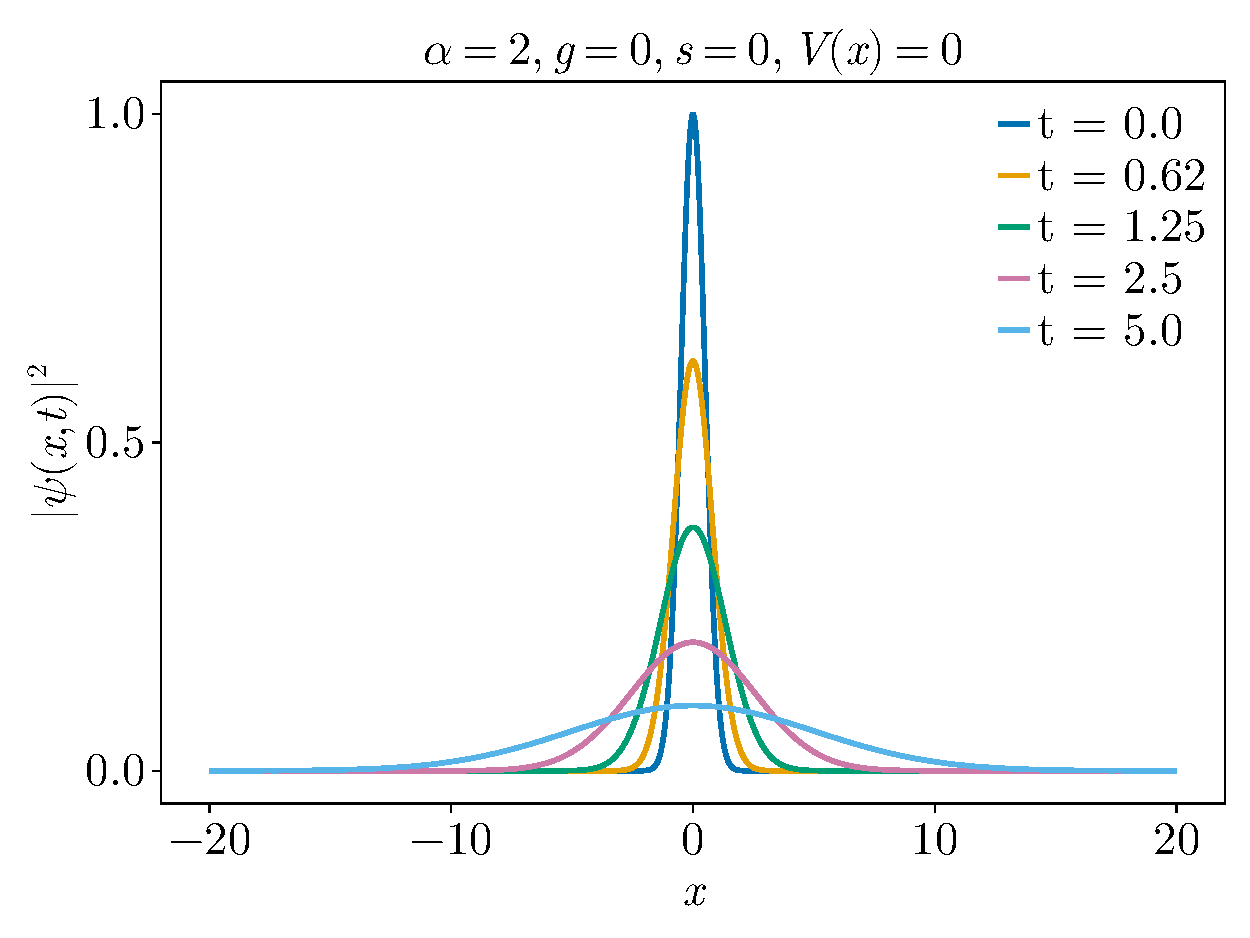
\includegraphics[width=\linewidth]{../figs/lse_evolution.pdf}
	\caption{Numerical simulation - Evolution of wave function $\psi_0$}
	\label{fig:lse_evolution}
\end{figure}
\begin{figure}[h!]
	\centering
	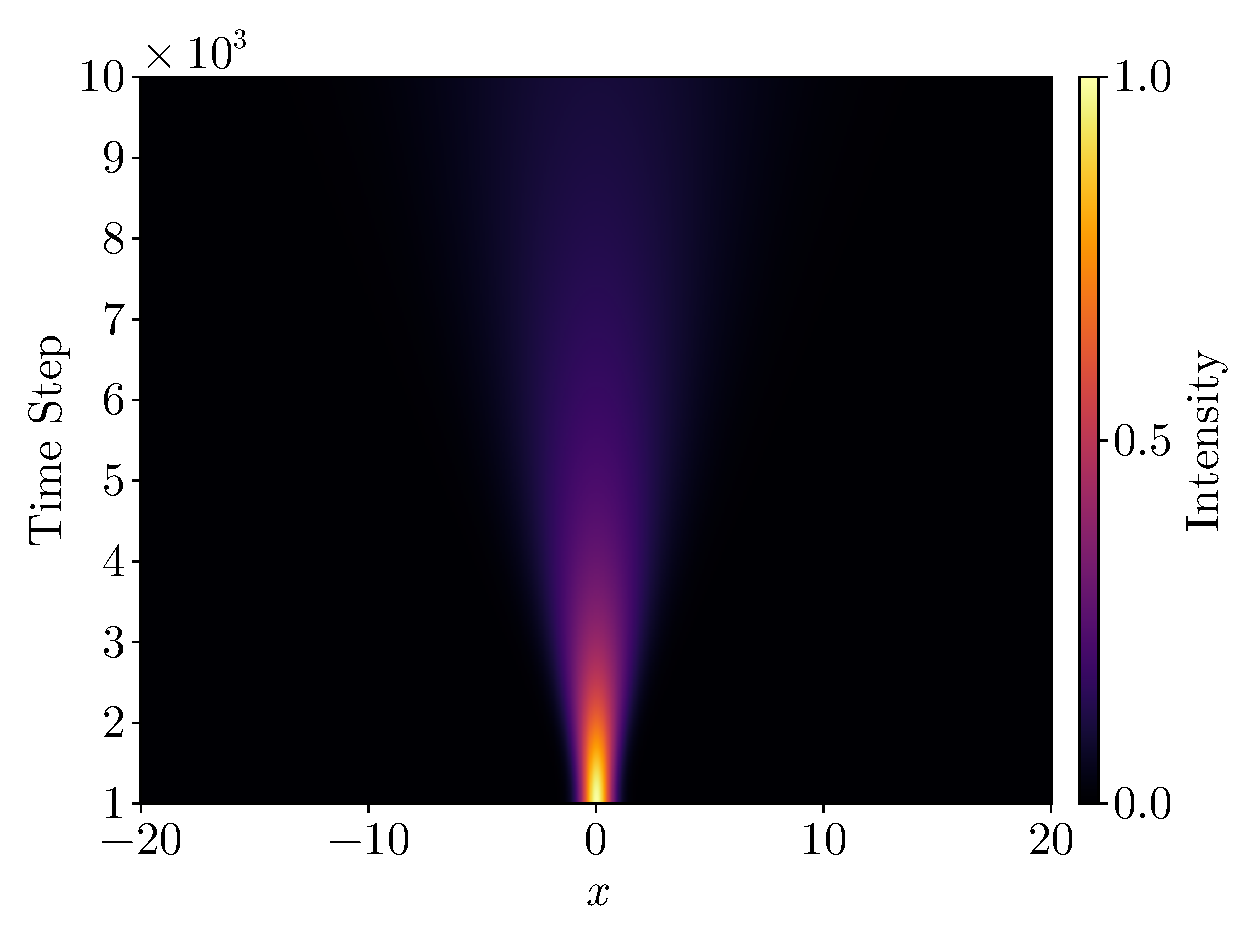
\includegraphics[width=\linewidth]{../figs/lse_heatmap.pdf}
	\caption{Numerical simulation - Heatmap of the evolution of wave function $\psi_0$}
	\label{fig:lse_heatmap}
\end{figure}
As seen in the figures \ref{fig:lse_evolution} and \ref{fig:lse_heatmap}, the numerical simulation of the Linear Schrödinger Equation (LSE) shows
a dispersing Gaussian wave packet. The wave packet spreads out over time, consistent with the 
analytical solution. Additionally, The heatmap provides a visual representation of the wave packet's evolution,
showing the dispersion of the wave function as time progresses.\\

The exact solution to this problem, when starting with a Gaussian initial condition, $\psi_0(x) = e^{-x^2}$, 
is known to be a \textbf{dispersing Gaussian wave packet}. For the free particle Schrödinger equation, the 
time-evolved solution \cite{shankar2012principles} for a Gaussian wave packet is:
\begin{equation}
    \psi(x,t) = \frac{1}{\sqrt{1 + 2it}} \exp\left(- \frac{x^2}{1 + 2it}\right)
\end{equation}
\begin{figure}[h!]
	\centering
	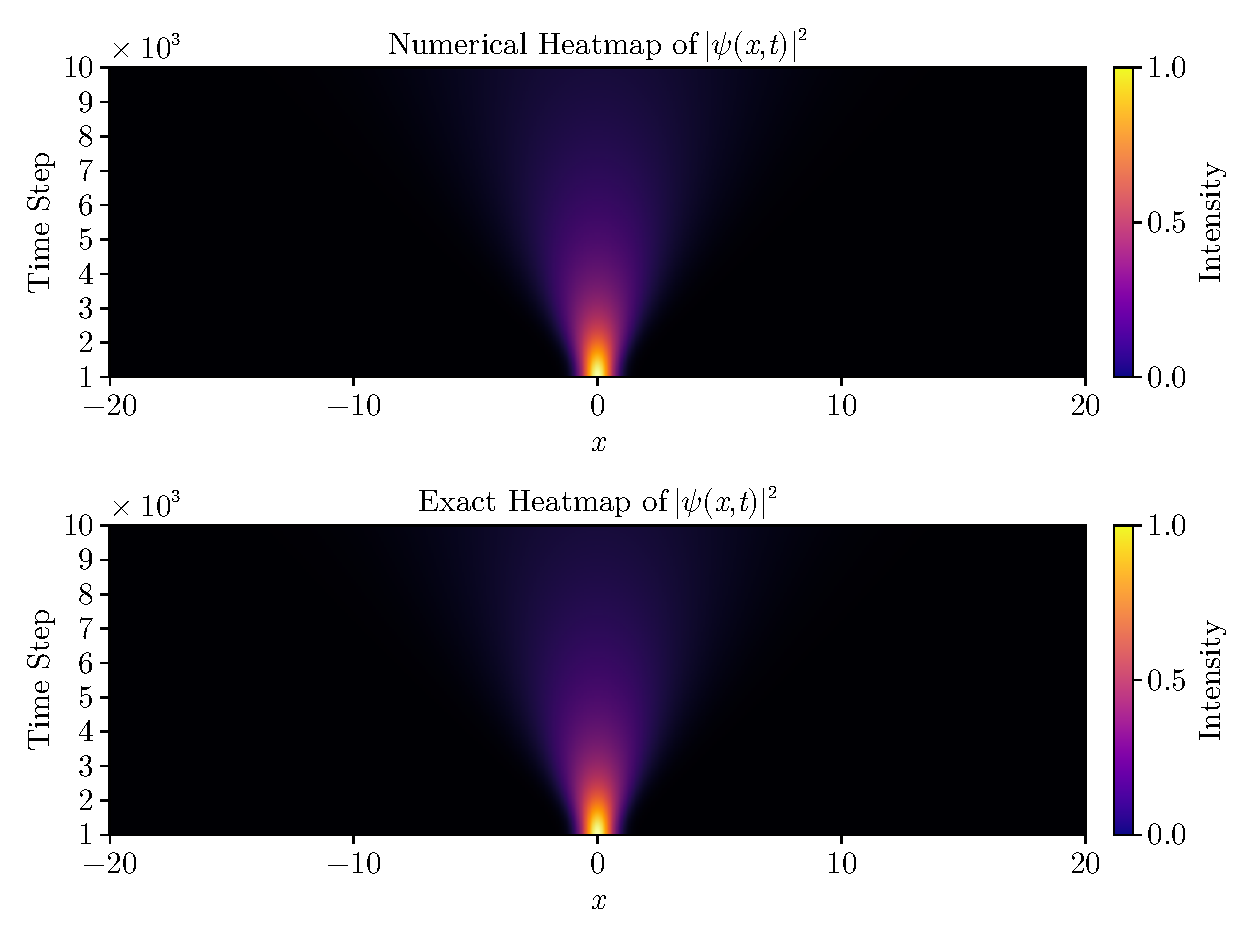
\includegraphics[width=\linewidth]{../figs/lse_comparison_heatmap.pdf}
	\caption{Comparison of Numerical and Analytical solutions of the wave function $\psi_0$}
	\label{fig:lse_comparison_heatmap}
\end{figure}
\begin{itemize}
	\item The Gaussian wave packet remains Gaussian at any later time, but it spreads 
	out, meaning the width of the wave packet increases as time progresses.
	\item The phase of the wave function will evolve over time, as indicated by 
	the imaginary part in the time-evolved solution.
\end{itemize}


This describes the spreading (dispersing) of the initial Gaussian wave packet over time.
\begin{figure}[h!]
	\centering
	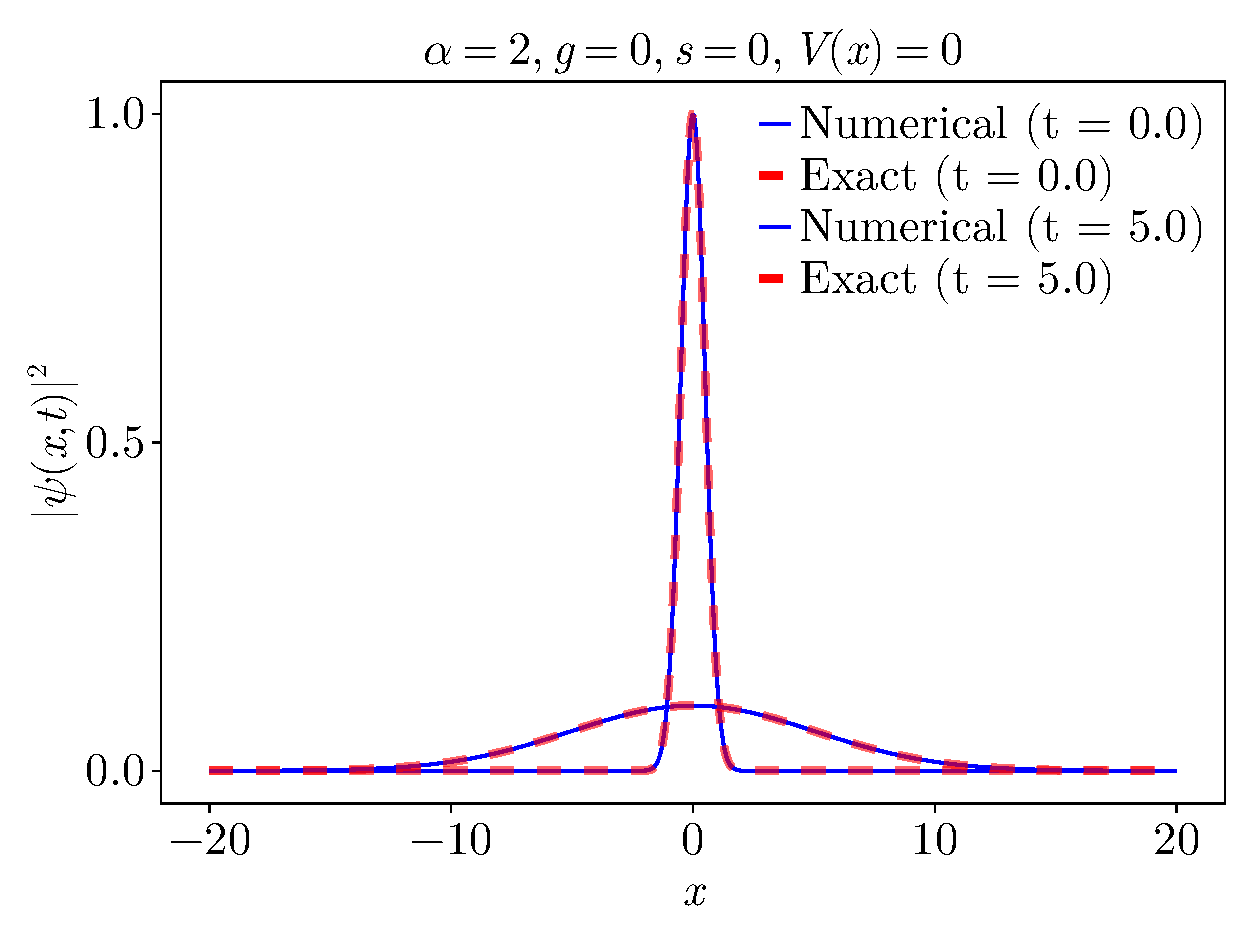
\includegraphics[width=\linewidth]{../figs/lse_comparison_lineplot.pdf}
	\caption{Comparison of Numerical and Analytical solutions of the wave function $\psi_0$}
	\label{fig:lse_comparison_lineplot}
\end{figure}

To further affirm and check the results, I plotted the Numerical and Analytical solutions of the wave 
function together to compare the results. As one can observe in the figure 
\ref{fig:lse_comparison_heatmap}, and the line plot in figure \ref{fig:lse_comparison_lineplot}, 
the numerical solution and the exact solution are in excellent agreement, confirming the 
correctness of the implementation.


\subsection{Nonlinear Schrödinger Equation (NLSE)}

\begin{table}[h!]
	\centering
	\begin{tabular}{c|c}
	\toprule
	\textbf{Description} & \textbf{Value}     \\ 
	\midrule
	Number of spatial points ($N$)              & 1000              \\ 
	Final time ($t_{\text{final}}$)             & [5.0, 20.0]       \\ 
	Time step ($dt$)                            & 0.0005            \\ 
	Total number of time steps ($M$)            & 10000             \\ 
	Spatial domain length ($L$)                 & 50.0              \\ 
	Spatial grid range ($x_{\text{grid}}$)      & [-20.0, 20.0]     \\
	Nonlinearity activation parameter ($g$)     & 1.0               \\
	Saturation parameter ($s$)                  & 1.0               \\
	\bottomrule
	\end{tabular}
	\caption{Parameters used in the numerical simulation.}
\end{table}

In this case, I am solving a time-dependent Nonlinear Schrödinger
equation with nonlinearity, potential, and saturation all set to one. Additionally, I am setting the
$\alpha = 2$ to neglect the fractional derivative term. The equation becomes:

\begin{equation}
	i \frac{\partial \psi}{\partial t} = \left[ \frac{1}{2} \left( - \frac{\partial^2}
	{\partial x^2}\right) - |\psi|^2 + V(x) \right] \psi
\end{equation}
Along with this, the initial wavepacket is a travelling soliton with a Gaussian profile. The 
soliton is
\begin{equation}
	\psi(x, 0) = \exp{(x^2 + ix)}
	\label{eq:initial_wavepacket}
\end{equation}

As seen in the figures \ref{fig:nlse_evolution} and \ref{fig:nlse_heatmap}, the numerical 
simulation of the Nonlinear Schrödinger Equation (NLSE) shows no interesting behavior. The wave 
packet travels but the spreading is more faster than the linear case. Now, let's make things interesting by manipulating the parameters $g$ and $s$ and add some nice 
potentials.
\begin{figure}[h!]
	\centering
	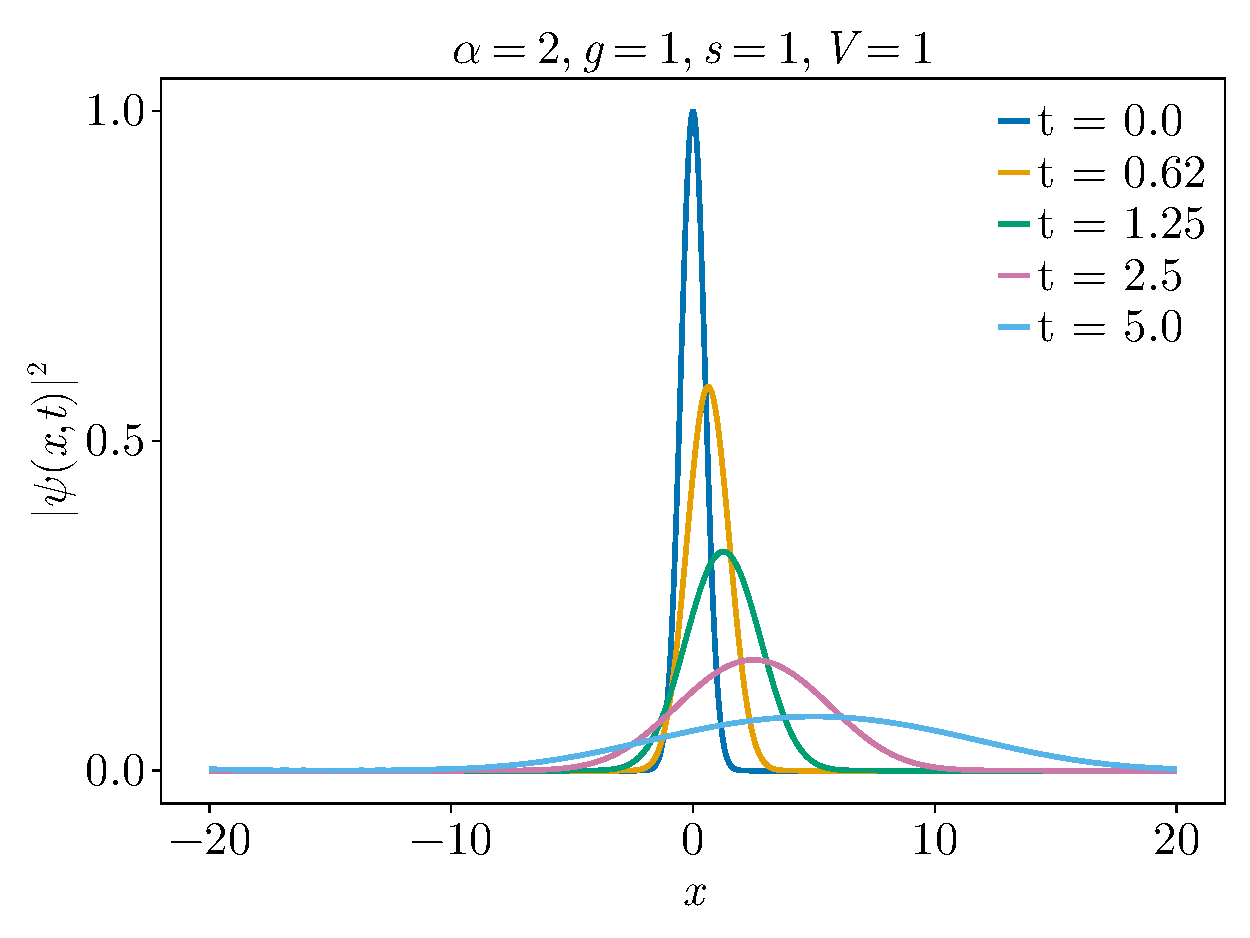
\includegraphics[width=\linewidth]{../figs/nlse_evolution_00.pdf}
	\caption{Numerical simulation - Evolution of wave function $\psi_0$}
	\label{fig:nlse_evolution}
\end{figure}
\begin{figure}[h!]
	\centering
	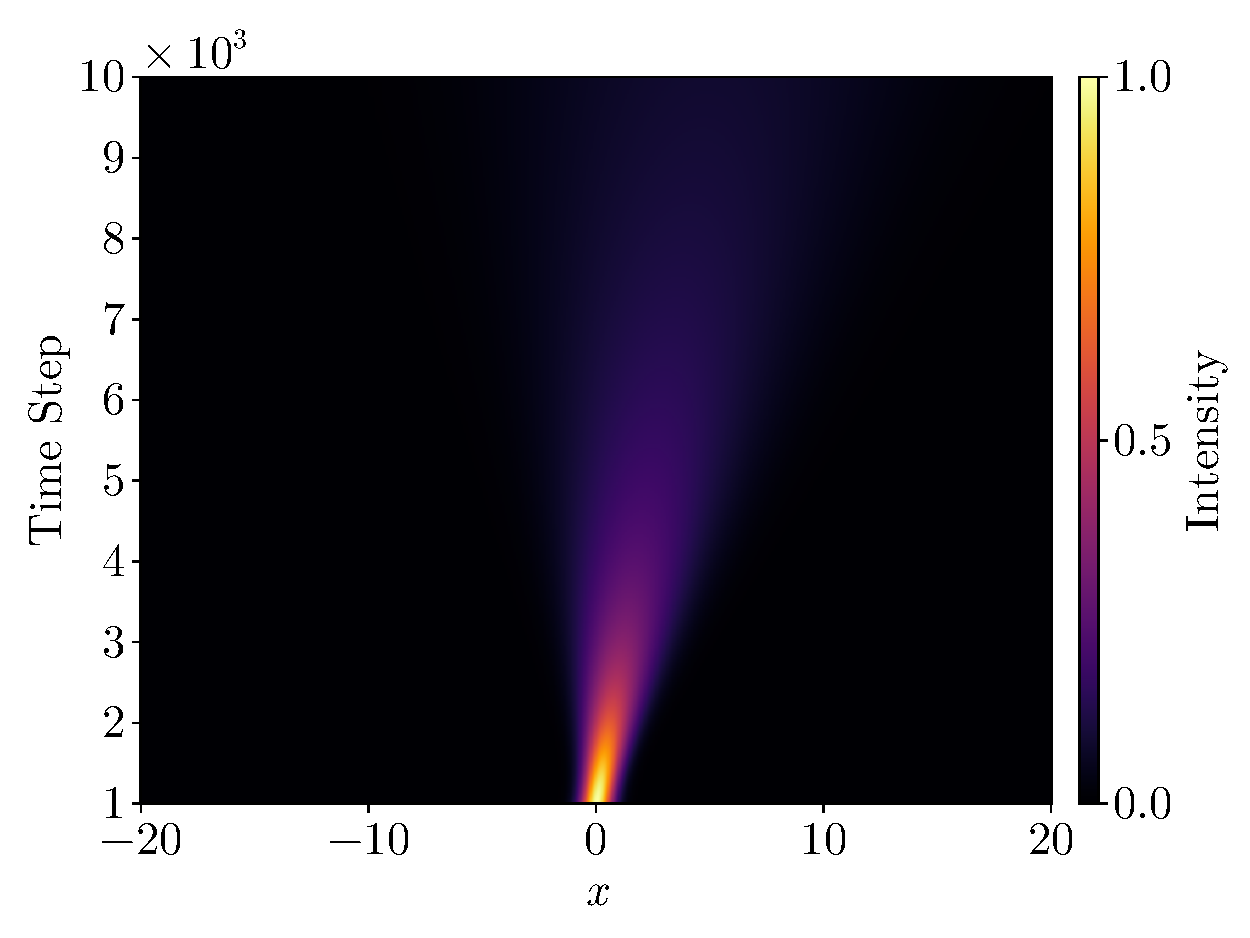
\includegraphics[width=\linewidth]{../figs/nlse_heatmap_00.pdf}
	\caption{Numerical simulation - Heatmap of the evolution of wave function $\psi_0$}
	\label{fig:nlse_heatmap}
\end{figure}
\subsubsection{Effect of Step Potential}
\begin{figure}[h!]
	\vspace{-3.5ex}
	\centering
	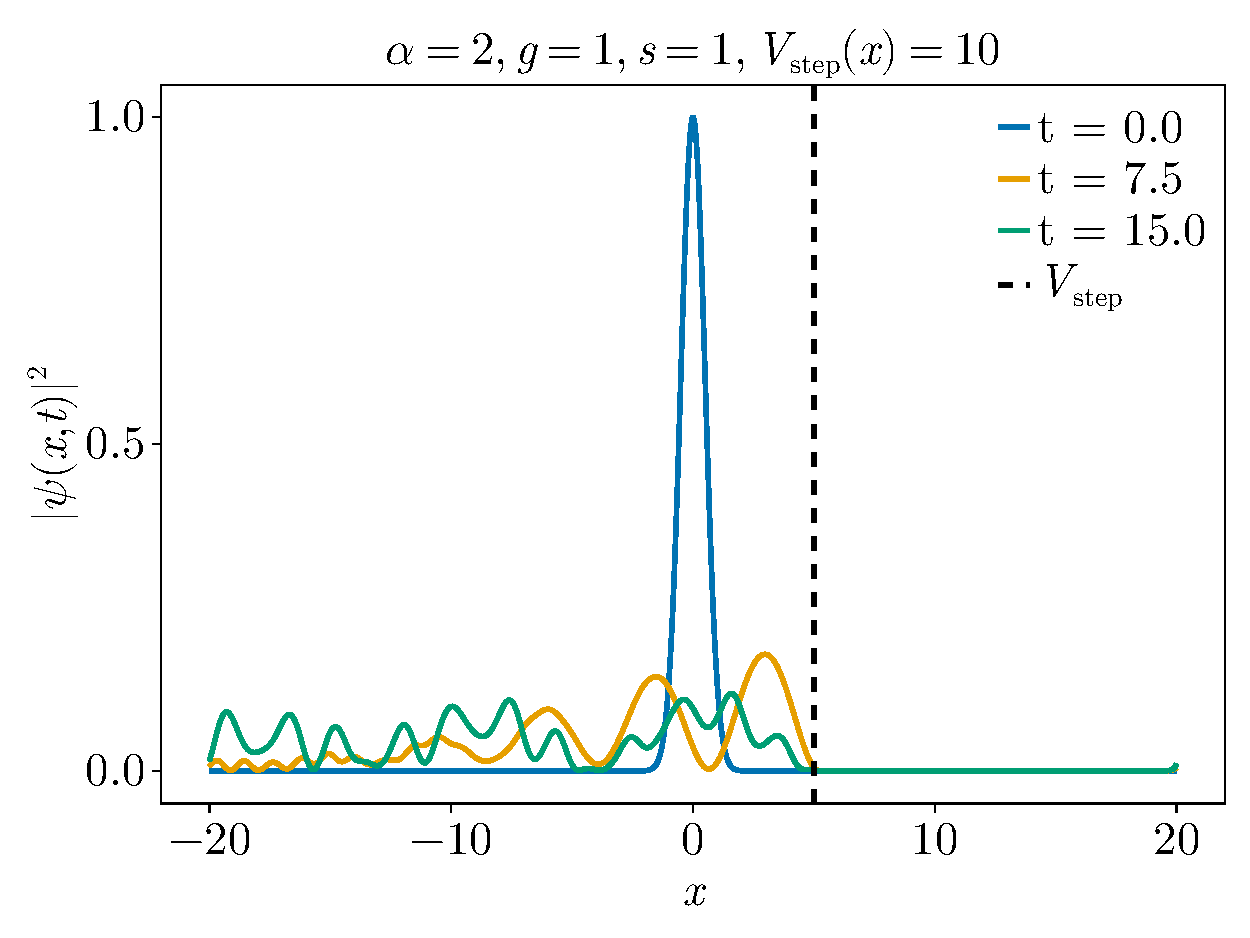
\includegraphics[width=\linewidth]{../figs/nlse_evolution_step.pdf}
	\caption{Numerical simulation - Evolution of wave function $\psi_0$ with step potential}
	\label{fig:nlse_evolution_step}
\end{figure}
\begin{figure}[h!]
	\vspace{-3.5ex}
	\centering
	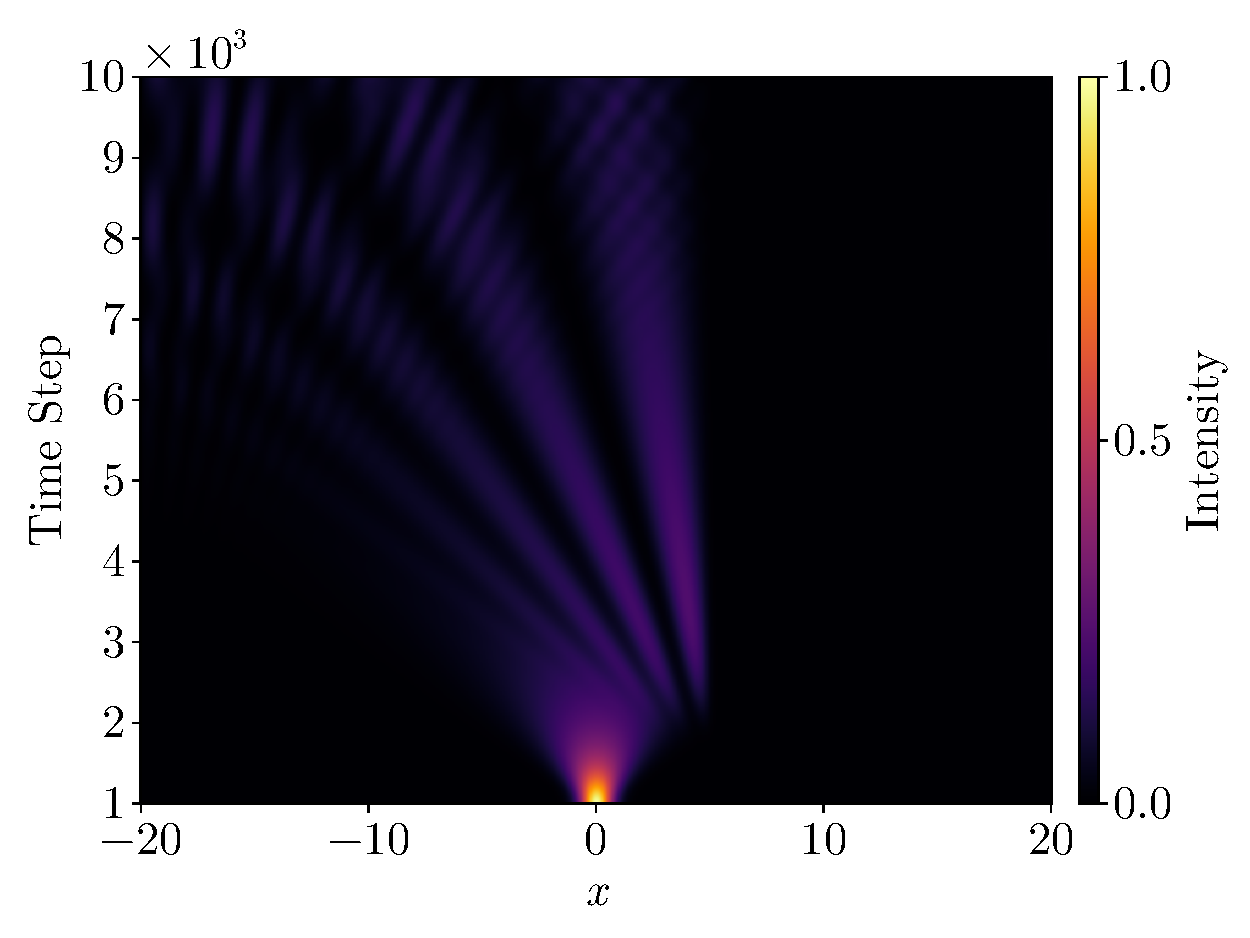
\includegraphics[width=\linewidth]{../figs/nlse_heatmap_step.pdf}
	\caption{Numerical simulation - Heatmap of the evolution of wave function $\psi_0$ with step potential}
	\label{fig:nlse_heatmap_step}
\end{figure}
\begin{equation}
	V(x) = \begin{cases}
		0, & \text{if } x < 5 \\
		10, & \text{if } x \geq 5
	\end{cases}
\end{equation}
I implemented a step potential in the simulation to observe the effect of the potential on the wave
which can be seen in the figures \ref{fig:nlse_evolution_step} and \ref{fig:nlse_heatmap_step}. Since $V(x) = 10$ is significantly higher than the wave packet’s energy, most of the wave packet 
gets reflected back, forming an interference pattern between the incoming and reflected waves. 
This results in sharp oscillations, where the amplitude oscillates rapidly due to constructive and 
destructive interference.


\subsubsection{Effect of Harmonic Potential}
\begin{equation}
	V(x) = x^2
\end{equation}
I implemented a harmonic potential in the simulation to observe the effect of the potential on the 
wave which can be seen in the figures \ref{fig:nlse_evolution_harmonic} and 
\ref{fig:nlse_heatmap_harmonic}.
\begin{figure}[h!]
	\centering
	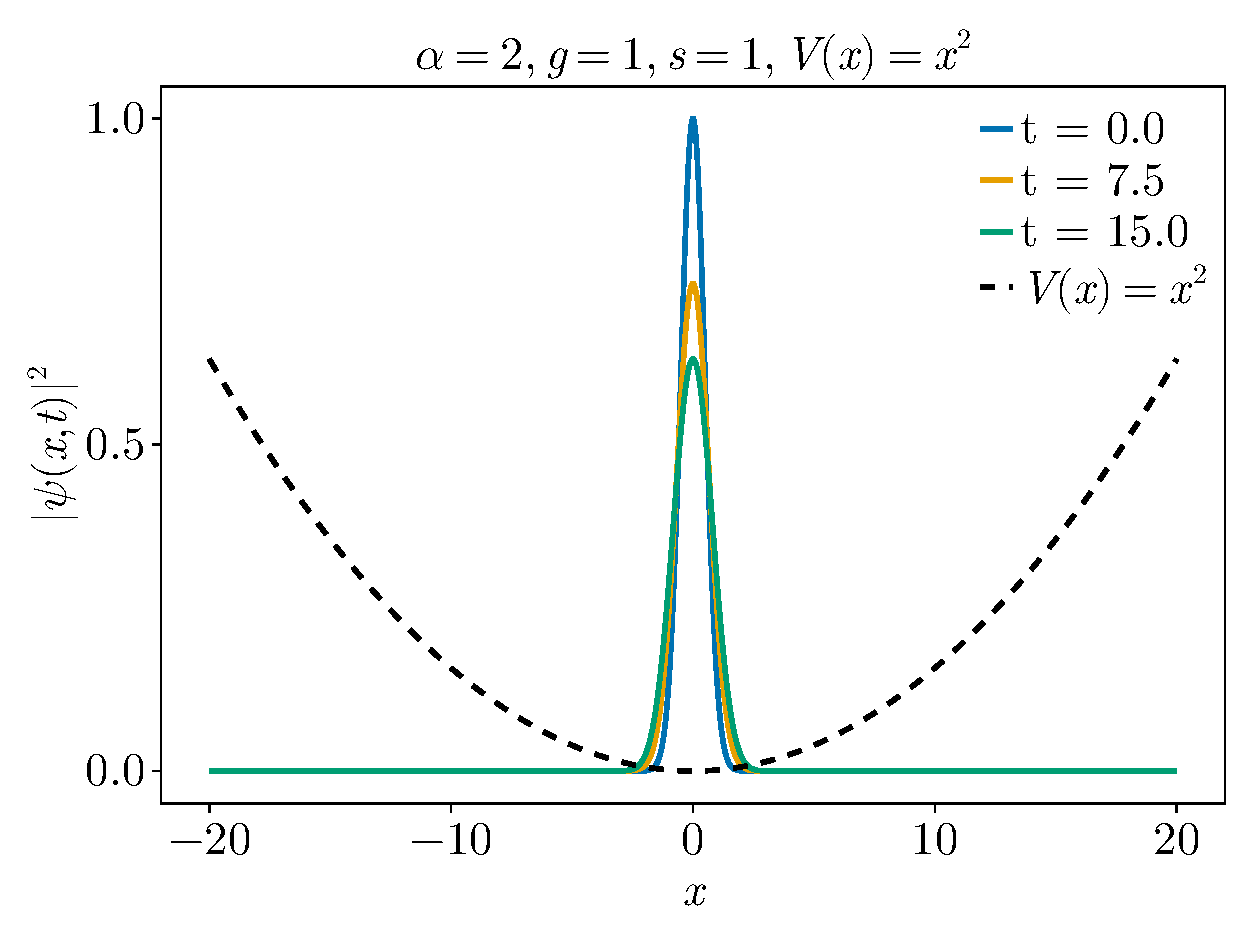
\includegraphics[width=\linewidth]{../figs/nlse_evolution_harmonic.pdf}
	\caption{Numerical simulation - Evolution of wave function $\psi_0$ with harmonic potential}
	\label{fig:nlse_evolution_harmonic}
\end{figure}
\begin{figure}[h!]
	\centering
	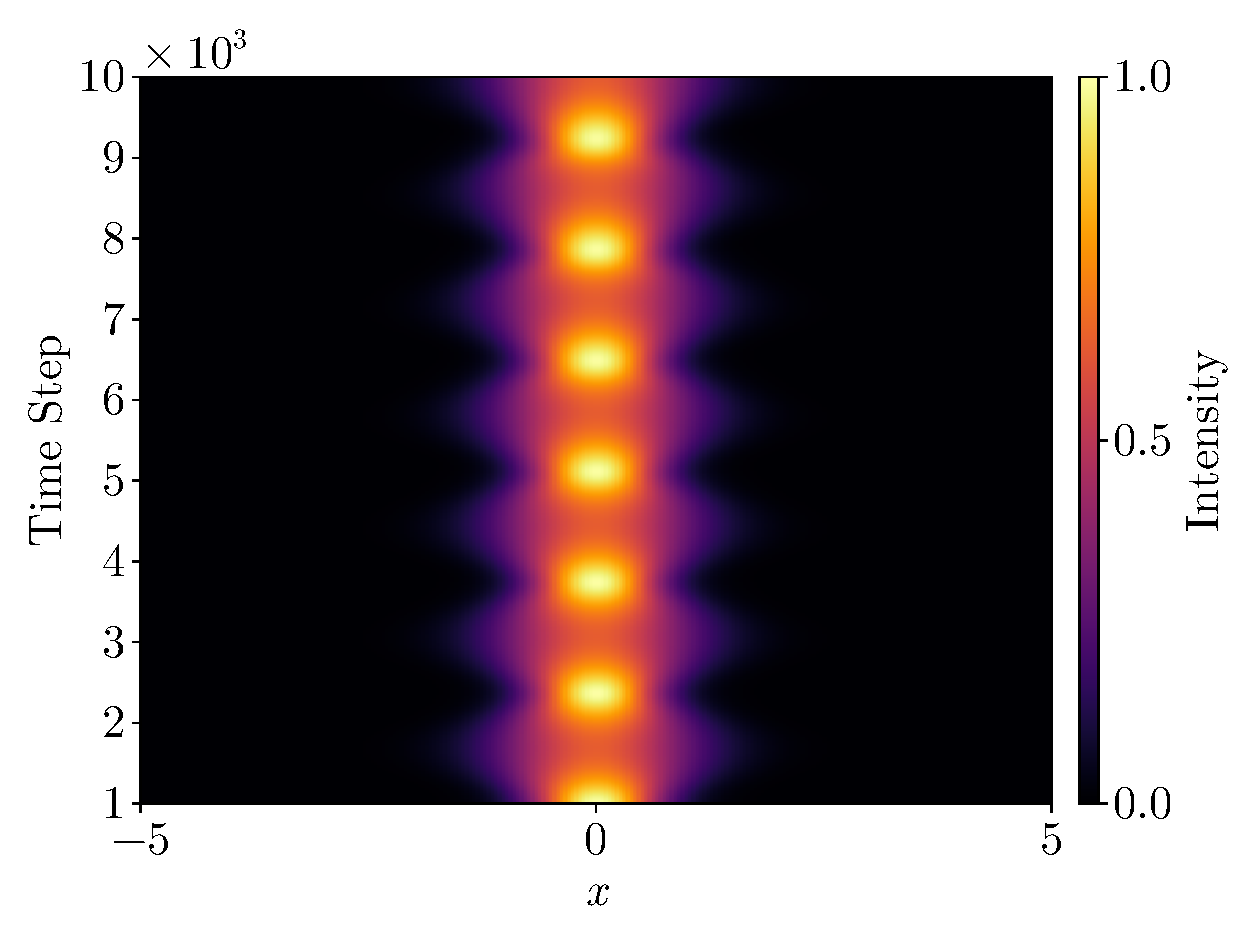
\includegraphics[width=\linewidth]{../figs/nlse_heatmap_harmonic.pdf}
	\caption{Numerical simulation - Heatmap of the evolution of wave function $\psi_0$ with harmonic potential}
	\label{fig:nlse_heatmap_harmonic}
\end{figure}

The harmonic potential $V(x) = x^2$ acts as a restoring force, confining the wave packet to the
center of the potential well. The wave packet oscillates back and forth within the well,
exhibiting a harmonic motion. Hence, these type of oscillations
are also called \textbf{breather solutions} in the context of Nonlinear Schrödinger Equation (NLSE).
\subsection{Normalized Nonlinear Fractional Schrödinger Equation (NNFSE)}
Finally, I implemented the evolution of Normalized Nonlinear Fractional Schrödinger Equation (NNFSE) with different 
values of $\alpha$ to observe the effect of fractional derivatives on the wave function. 
\begin{table}[h!]
	\centering
	\begin{tabular}{c|c}
	\toprule
	\textbf{Description} & \textbf{Value}     \\ 
	\midrule
	Number of spatial points ($N$)              & 1000              \\ 
	Final time ($t_{\text{final}}$)             & [5.0, 15, 20.0]   \\ 
	Time step ($dt$)                            & 0.0005            \\ 
	Total number of time steps ($M$)            & 10000             \\ 
	Spatial domain length ($L$)                 & 50.0              \\ 
	Spatial grid range ($x_{\text{grid}}$)      & [-20.0, 20.0]     \\
	Nonlinearity activation parameter ($g$)     & [1.0, 2]          \\
	Saturation parameter ($s$)                  & [1.0, 1.5]        \\
	\bottomrule
	\end{tabular}
	\caption{Parameters used in the numerical simulation.}
\end{table}

The initial wavepacket is the same \ref{eq:initial_wavepacket}, a travelling 
soliton with a Gaussian profile.

\subsubsection{Effect of Fractional Derivative ($\alpha = 1.2$)}

\begin{figure}[h!]
	\centering
	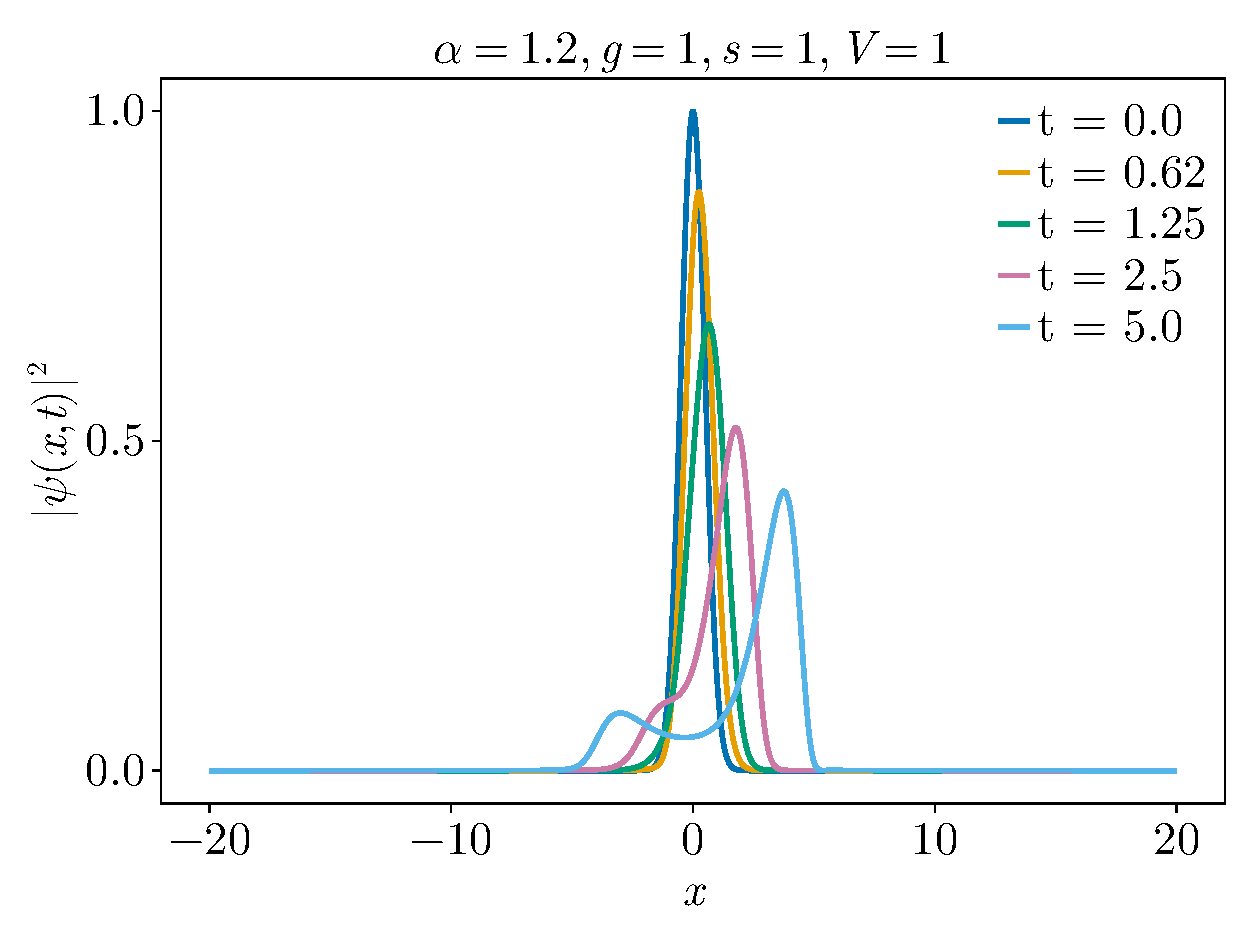
\includegraphics[width=\linewidth]{../figs/fnlse_evolution_00.pdf}
	\caption{Numerical simulation - Evolution of wave function $\psi_0$}
	\label{fig:nnfse_evolution_alpha00}
\end{figure}
\begin{figure}[h!]
	\centering
	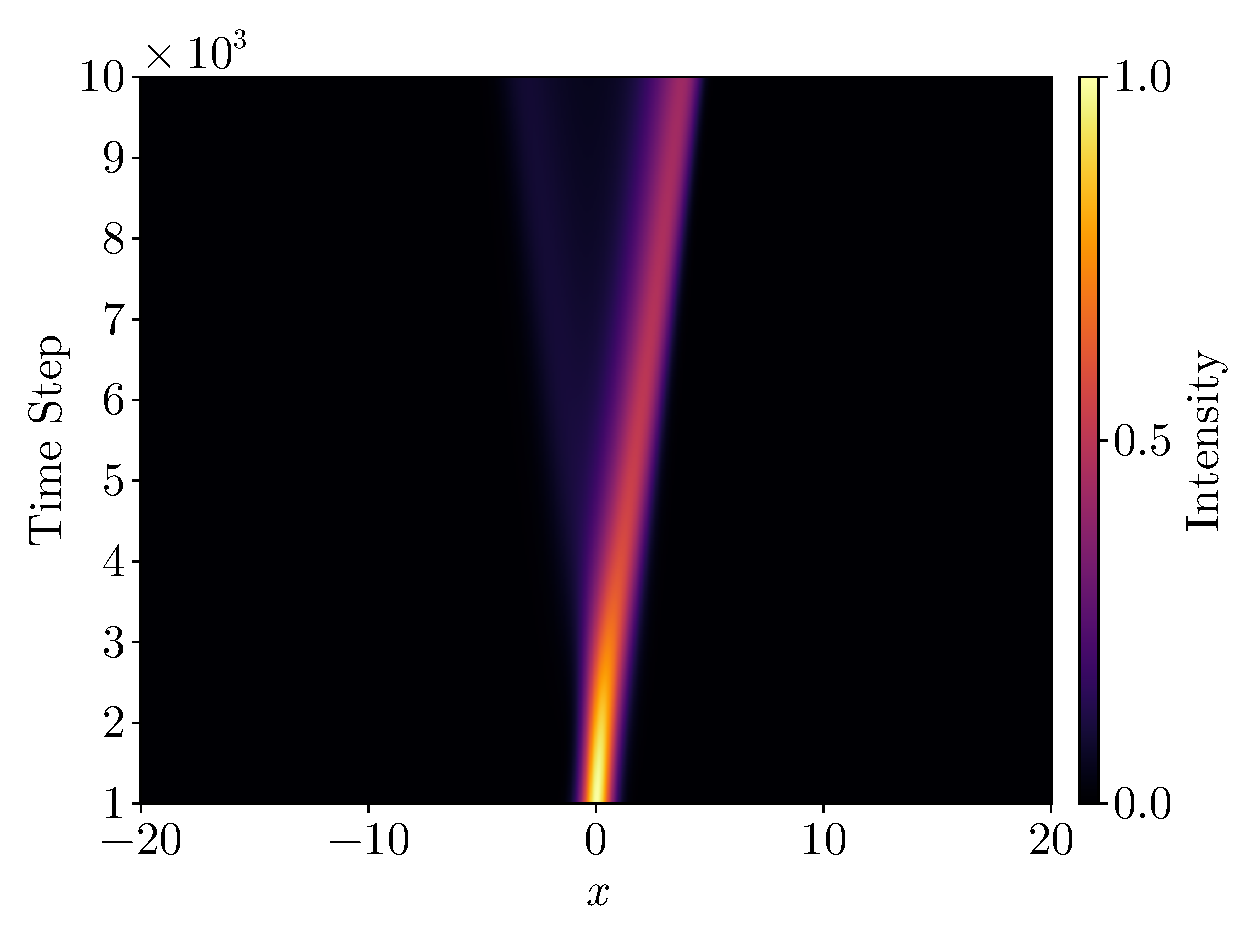
\includegraphics[width=\linewidth]{../figs/fnlse_heatmap_00.pdf}
	\caption{Numerical simulation - Heatmap of the evolution of wave function $\psi_0$}
	\label{fig:nnfse_heatmap_alpha00}
\end{figure}

As seen in the figures \ref{fig:nnfse_evolution_alpha00} and \ref{fig:nnfse_heatmap_alpha00}, The
wave packet is sharp and does not disperse as much as the linear case. 

\subsubsection{Effect of Fractional Derivative ($\alpha = 1.5$)}

\begin{figure}[h!]
	\centering
	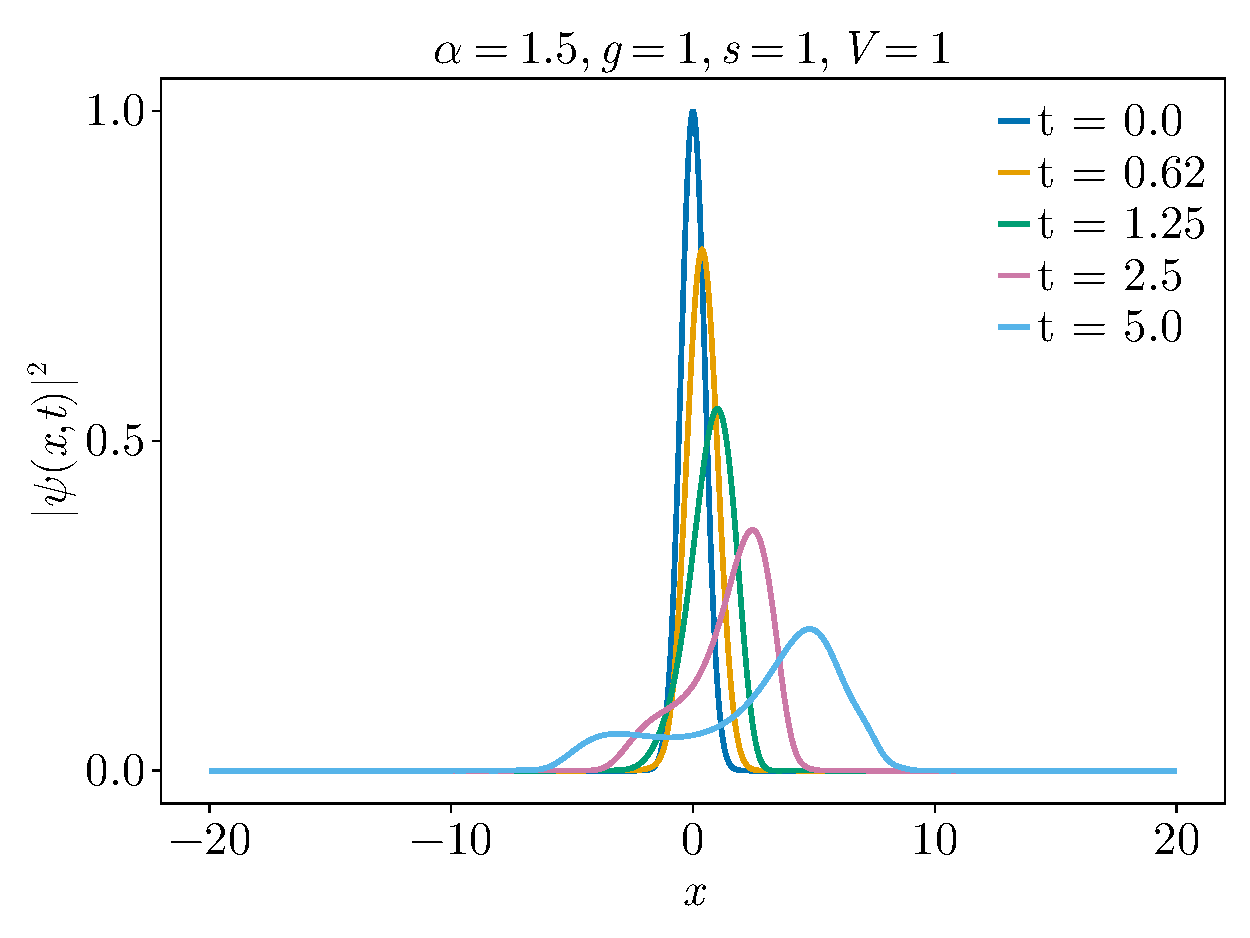
\includegraphics[width=\linewidth]{../figs/fnlse_evolution_01.pdf}
	\caption{Numerical simulation - Evolution of wave function $\psi_0$}
	\label{fig:nnfse_evolution_alpha01}
\end{figure}
\begin{figure}[h!]
	\centering
	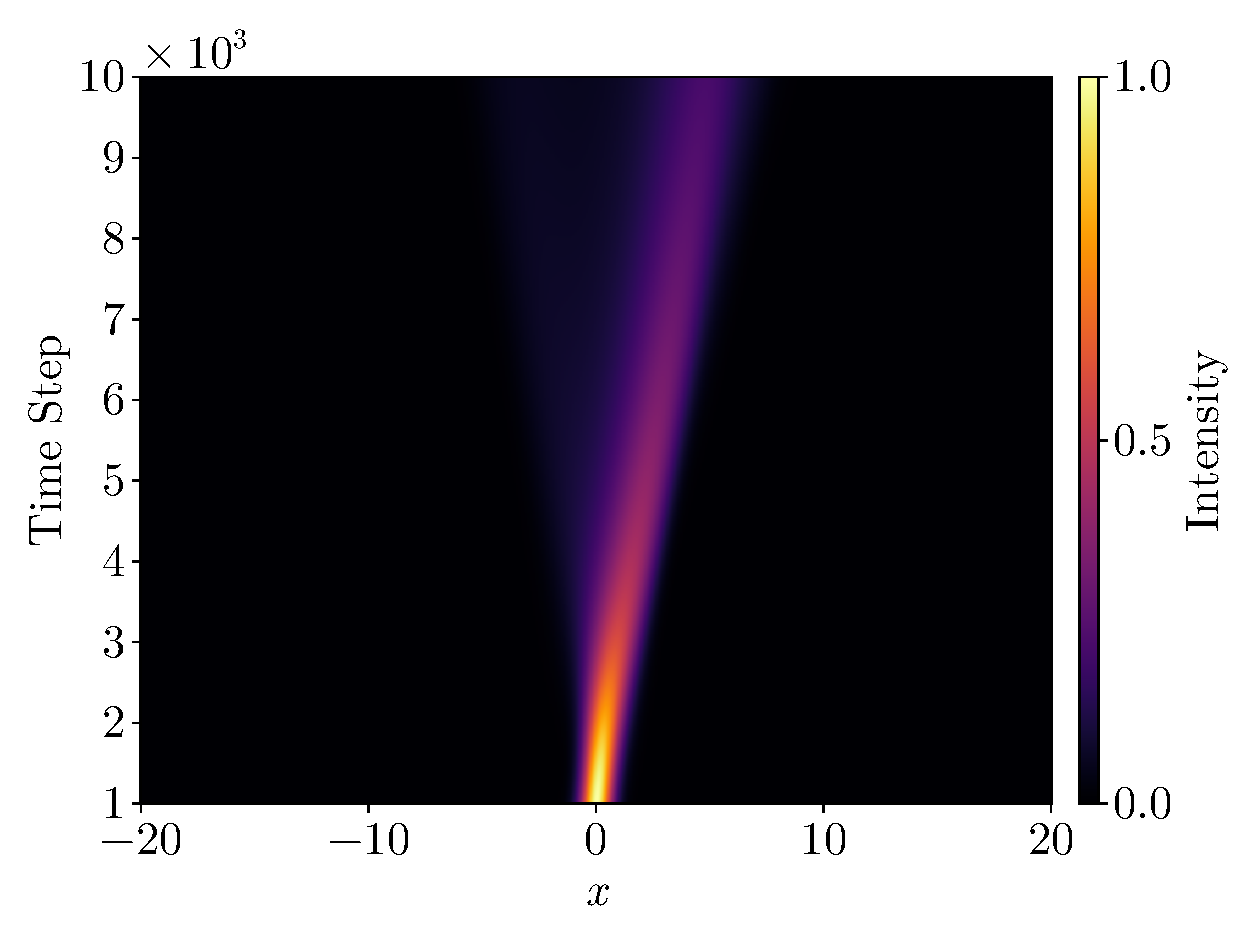
\includegraphics[width=\linewidth]{../figs/fnlse_heatmap_01.pdf}
	\caption{Numerical simulation - Heatmap of the evolution of wave function $\psi_0$}
	\label{fig:nnfse_heatmap_alpha01}
\end{figure}

As seen in the figures \ref{fig:nnfse_evolution_alpha01} and \ref{fig:nnfse_heatmap_alpha01}, The
wave packet starts dispersing faster now as it should because as the value of alpha increases it 
starts behaving more like the normal Schrödinger equation.

\subsubsection{Effect of Fractional Derivative ($\alpha = 1.8$)}

\begin{figure}[h!]
	\centering
	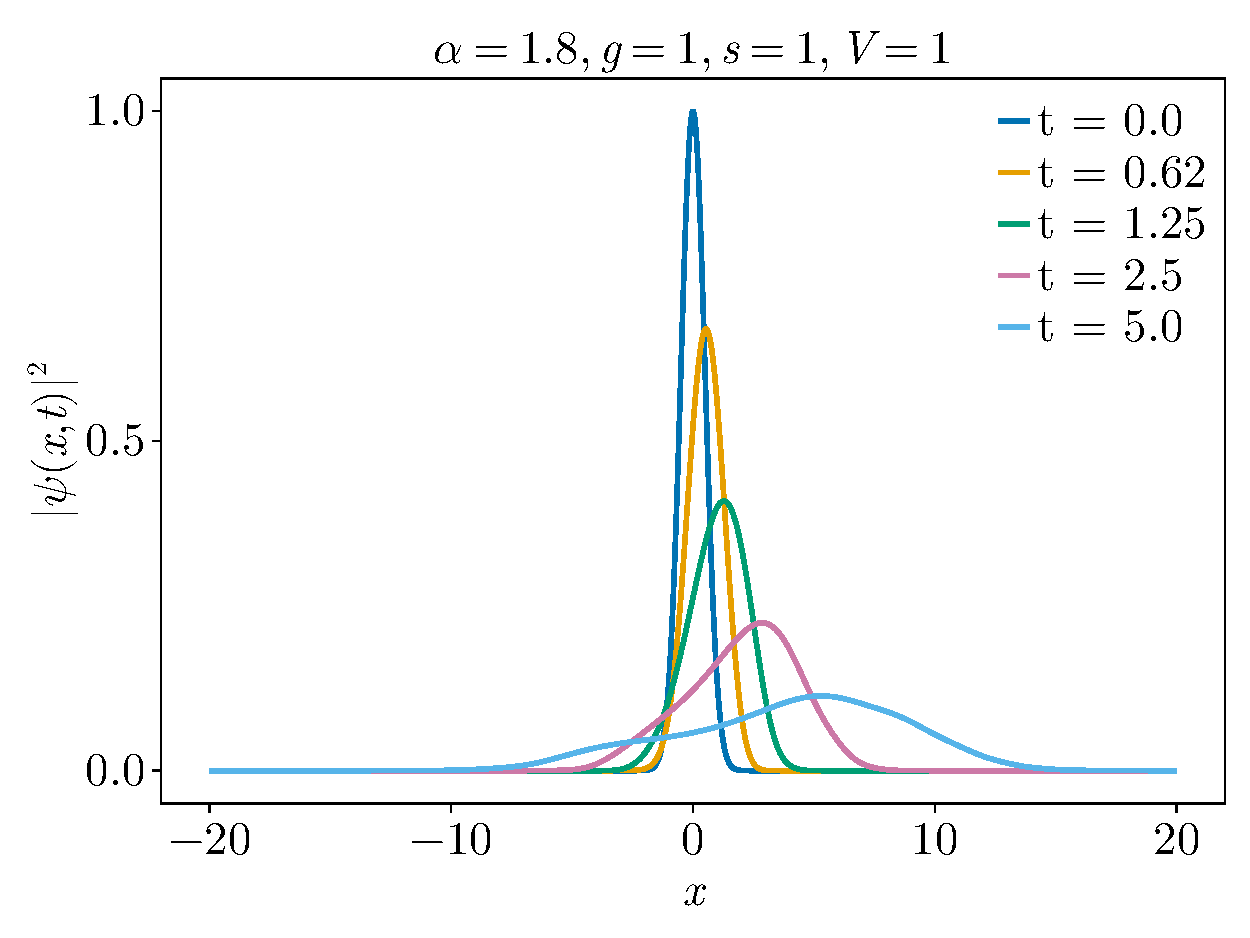
\includegraphics[width=\linewidth]{../figs/fnlse_evolution_02.pdf}
	\caption{Numerical simulation - Evolution of wave function $\psi_0$}
	\label{fig:nnfse_evolution_alpha02}
\end{figure}
\begin{figure}[h!]
	\centering
	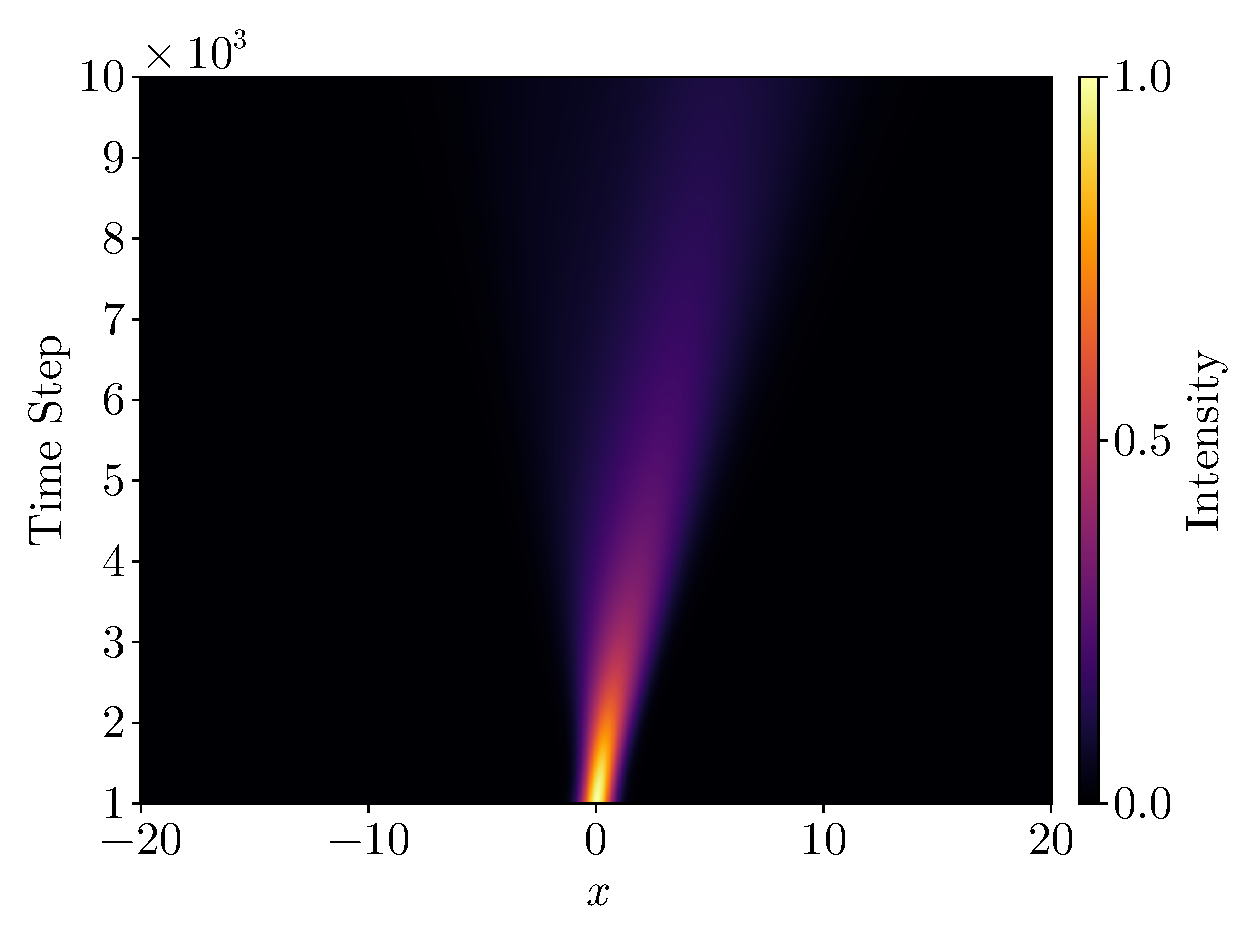
\includegraphics[width=\linewidth]{../figs/fnlse_heatmap_02.pdf}
	\caption{Numerical simulation - Heatmap of the evolution of wave function $\psi_0$}
	\label{fig:nnfse_heatmap_alpha02}
\end{figure}

The wave packet is dispersing faster now as the value of $\alpha$ is closer to 2. This once again confirms
the correctness of the implementation. This can be observed in the figures \ref{fig:nnfse_evolution_alpha02} and
\ref{fig:nnfse_heatmap_alpha02}.

\subsubsection{Effect of Harmonic Potential}

\begin{figure}[h!]
	\centering
	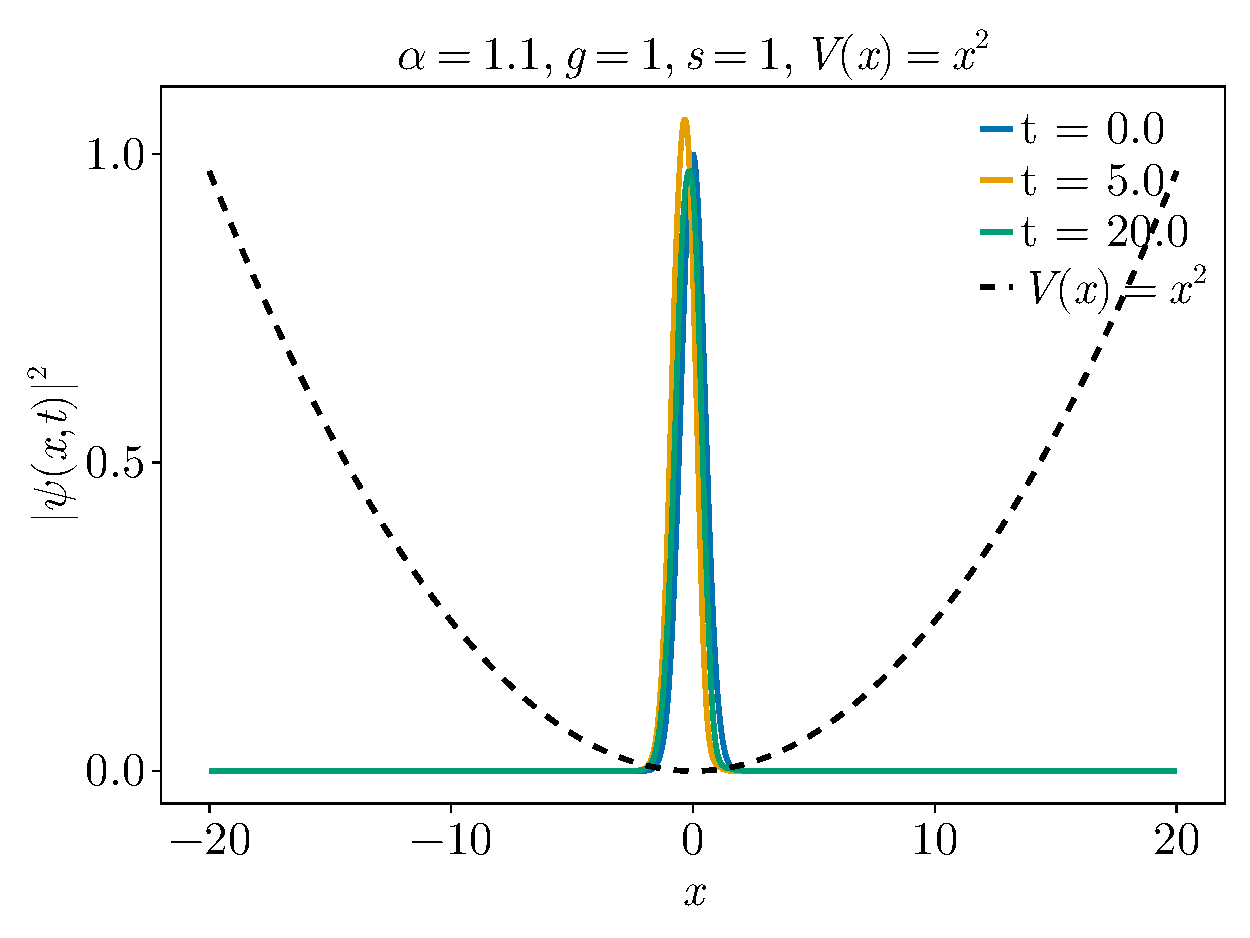
\includegraphics[width=\linewidth]{../figs/fnlse_evolution_har.pdf}
	\caption{Numerical simulation - Evolution of wave function $\psi_0$ with harmonic potential}
	\label{fig:nnfse_evolution_harmonic}
\end{figure}
\begin{figure}
	\centering
	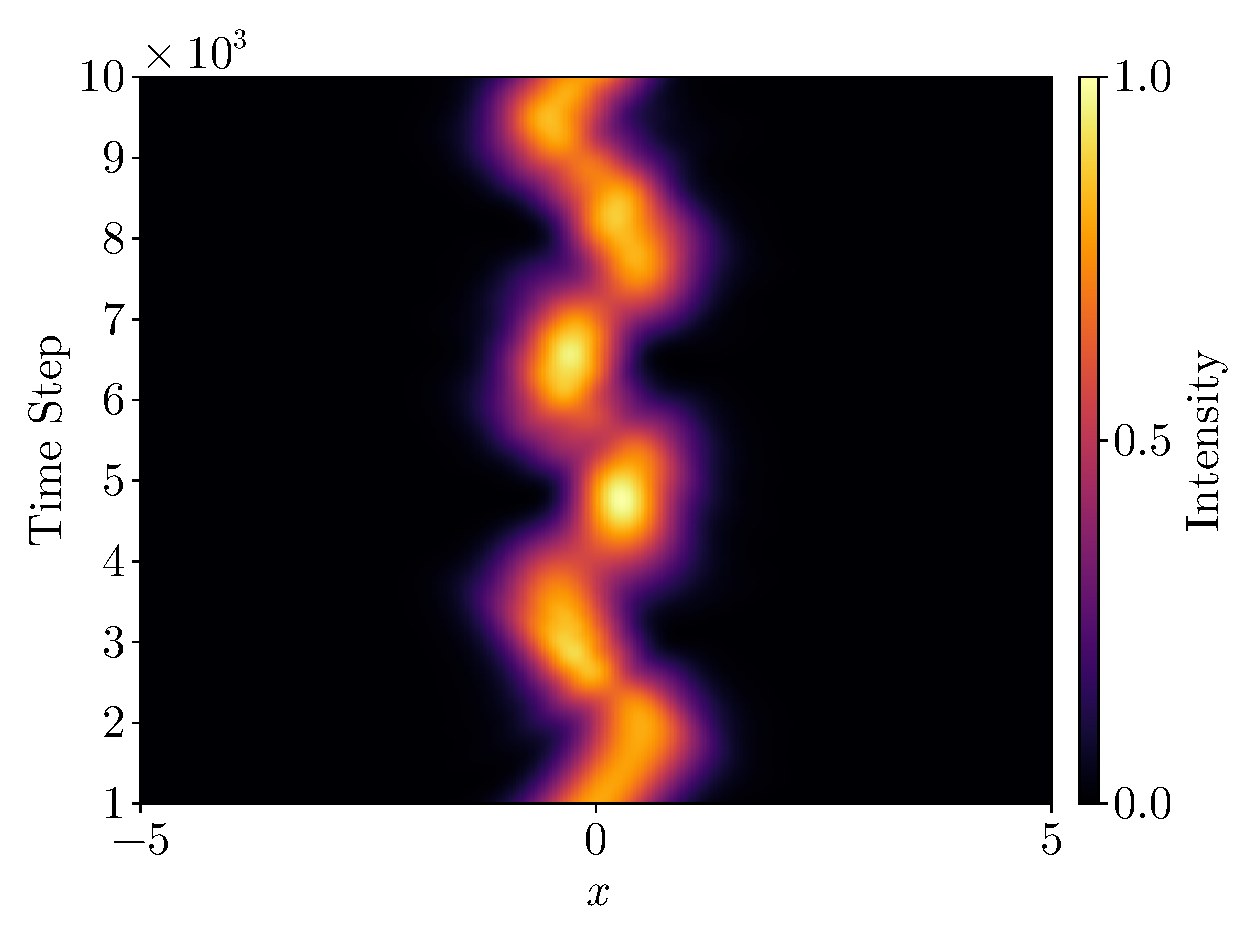
\includegraphics[width=\linewidth]{../figs/fnlse_heatmap_har.pdf}
	\caption{Numerical simulation - Heatmap of the evolution of wave function $\psi_0$ with harmonic potential}
	\label{fig:nnfse_heatmap_harmonic}
\end{figure}

Similar to what we observed in the NLSE simulations \ref{fig:nlse_evolution_harmonic} and \ref{fig:nlse_heatmap_harmonic}, The harmonic potential $V(x) = x^2$ acts as a restoring force, confining the wave packet to the
center of the potential well. This can be clearly seen in the figures \ref{fig:nnfse_evolution_harmonic} and
\ref{fig:nnfse_heatmap_harmonic}. Also, I changed $\alpha = 1.1$ to observe the effect of
fractional derivatives on the wave function. This makes it more fractional than other cases. The effect of this
can be observed as the oscillations are more erratic and spread out than the Nonlinear Schrödinger Equation (NLSE). Also the peaks are much sharper and the wave packet is more confined to the center of the 
potential well.


\subsubsection{Effect of Quartic Potential}

\begin{equation}
	V(x) = x^4
\end{equation}

I implemented a quartic potential in the simulation with $\alpha = 1.1$ and a stronger value of nonlinearity $g = 1$, 
and saturation $s = 1.5$ to observe the effect of the potential on the wave which can be seen in 
the figures \ref{fig:nnfse_evolution_quar} and \ref{fig:nnfse_heatmap_quar}.\\

\begin{figure}[h!]
	\centering
	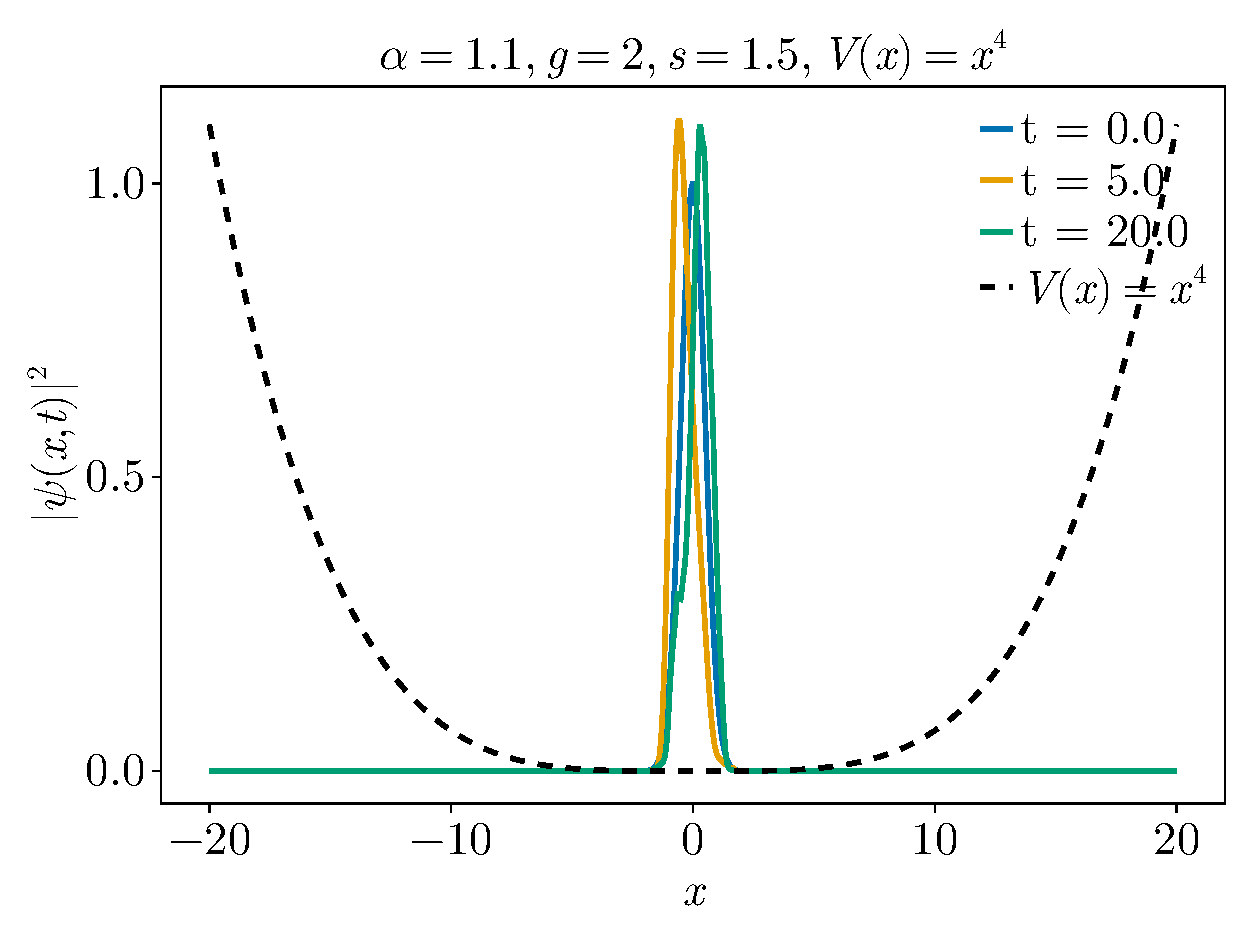
\includegraphics[width=\linewidth]{../figs/fnlse_evolution_quar.pdf}
	\caption{Numerical simulation - Evolution of wave function $\psi_0$ with quartic potential}
	\label{fig:nnfse_evolution_quar}
\end{figure}
\begin{figure}
	\centering
	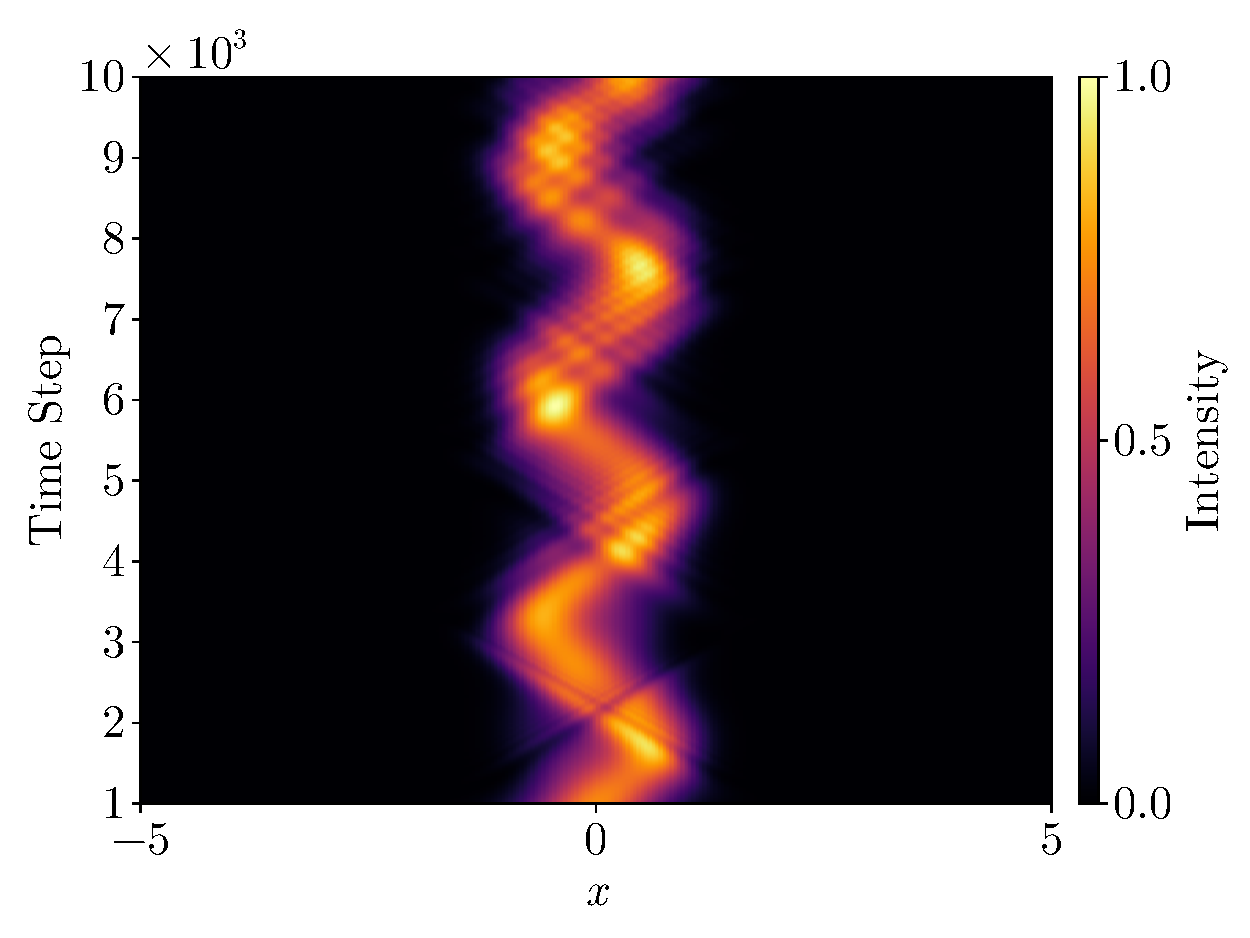
\includegraphics[width=\linewidth]{../figs/fnlse_heatmap_quar.pdf}
	\caption{Numerical simulation - Heatmap of the evolution of wave function $\psi_0$ with quartic potential}
	\label{fig:nnfse_heatmap_quar}
\end{figure}


This is more interesting to observe as I increase the value of nonlinearity and saturation, the wave packet
becomes more sharp and the oscillations are more erratic and spread out. The quartic potential acts as a
stronger restoring force, confining the wave packet to the center of the potential well. Also the combat between
the confining potential and strong nonlinearity and saturation can be clearly observed as there are constructive and 
destructive interference patterns forming in the wave packet in the heatmap.

\section{Conclusion}

In this project, I implemented the Split-Step Fourier Method (SSFM) to solve the Normalized Nonlinear Fractional
Schrödinger Equation (NNFSE). I started by solving the Linear Schrödinger Equation (LSE) to do a sanity check of the code.
Then I solved the Nonlinear Schrödinger Equation (NLSE) to observe the nonlinear behavior of the wave function. Finally, I solved
the NNFSE with different values of $\alpha$, $s$ and $g$, to observe the effect of fractional derivatives and saturation parameter.
The results show that the implementation is promising and the wave packet behaves as anticipated. The SSFM is an efficient
numerical technique for solving time-dependent nonlinear partial differential equations, providing insights into the
complex dynamics of wave phenomena. The project demonstrates the power of computational methods in exploring
nonlinear wave interactions and the impact of fractional derivatives on wave propagation. Future work could involve
extending the simulation to higher dimensions, exploring additional potential profiles, and investigating the
interplay between nonlinearity and dispersion in wave dynamics.\\

I would like to express my sincere gratitude to Prof. Dr. Johannes Berg for his invaluable guidance and 
support during this intensive week. The experience of working on the assigned tasks has been both 
enlightening and inspiring.\\

The code for this project can be found at \href{https://github.com/sahilugale/julia-intensive-week.git}{GitHub}.

\bibliographystyle{plain}
\bibliography{references}

\end{document}


